\documentclass{article}
\usepackage{graphicx} % Required for inserting images
\usepackage{subfigure}
\usepackage[a4paper, total={6in, 10in}]{geometry}

\title{\textbf{Titanic - survivor classification}}
\author{Łukasz Borak, Krzysztof Bryszak, Jakub Jagła, Maksymilian Żmuda-Trzebiatowski}
\date{April 2024}

\begin{document}

\maketitle

\section{Introduction}
\paragraph{} The sinking of the RMS Titanic on the 15th of April 1912 is the deadliest peacetime maritime disaster to date. Four days into her maiden voyage from Southampton to New York City, the ship struck an iceberg causing water to flood six to sixteen compartments. The ship sank completely in just below 3 hours, resulting in the death of more than 1500 people (crew and passengers).
\paragraph{} Throughout the years, after the disaster, numerous data have been collected regarding all of the ship’s passengers. Recently this collection of data has gathered significant attention from data scientists as a great starting point for novices in Machine Learning. The goal of this report is to find viable Data Mining techniques, which applied to the dataset will improve a classifier’s accuracy on the unseen part of the dataset.

\section{Dataset description}
\paragraph{}The Titanic dataset contains information about 1309 of the passengers present during the sinking. Each passenger is described with a variety of attributes, including their name, age, point of departure, ticket price, etc. Each passenger also has an assigned binary label, which describes whether they survived or not.

\newpage

\section{Input features}
\subsection{Feature descriptions}

\begin{itemize}
\item \textbf{PassengerId} - integer uniquely assigned to each row.
\item \textbf{Pclass} - integer describing the class of a passenger's ticket, i.e. first, second or third class.          
\item \textbf{Name} - name, surname, title and optionally a nickname of the passenger.
\item \textbf{Sex} - string describing the passenger's gender (male/female). 
\item \textbf{Age} - floating point number describing the passenger's age in years.     \item \textbf{SibSP} - integer describing the amount of passenger's siblings or spouses that were aboard.
\item \textbf{Parch} - integer describing the amount of passenger's parents or children that were aboard.     
\item \textbf{Ticket} - string describing the passenger's ticket number.
\item \textbf{Fare} - floating point number describing the fare paid for the ticket in dollars.
\item \textbf{Cabin} - string describing the passenger's cabin number. The numerical part is prefixed by a single character describing the deck level.
\item \textbf{Embarked} - a single character describing the port of embarkation.
\end{itemize}

\newpage
\subsection{Exploratory analysis of input features}
\paragraph{}In order to provide distributions with respect to target, EDA was performed on the training dataset of 891 records.
\begin{table}[htb]
\centering
\begin{tabular}{|l|l|l|l|}
\hline
\textbf{Column} & \textbf{NaNs} & \textbf{Mean} & \textbf{SD} \\ \hline
Pclass          & 0             & 2.31          & 0.84         \\ \hline
Name            & 0             & N/A           & N/A          \\ \hline
Sex             & 0             & N/A           & N/A          \\ \hline
Age             & 177           & 29.70         & 14.53        \\ \hline
SibSp           & 0             & 0.52          & 1.10         \\ \hline
Parch           & 0             & 0.38          & 0.81         \\ \hline
Ticket          & 0             & N/A           & N/A          \\ \hline
Fare            & 0             & 32.20         & 49.69        \\ \hline
Cabin           & 687           & N/A           & N/A          \\ \hline
Embarked        & 2             & N/A           & N/A          \\ \hline
\end{tabular}
\caption{Basic statistics for input features}
\end{table}
\paragraph{} A quick overview shows that most passengers' cabin number is missing. This could be because 3rd class passengers may not have been assigned specific cabins. There are also some values missing in the \textbf{Age} and \textbf{Embarked} columns.
\begin{figure}[htb]
    \centering
    \begin{subfigure}
        \centering
        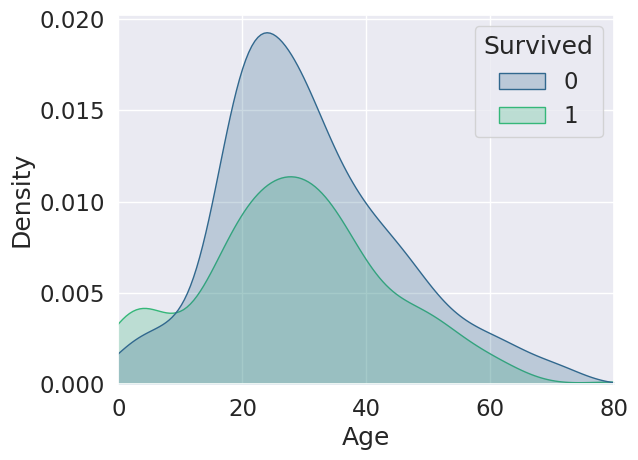
\includegraphics[width=0.49\linewidth]{age.png}
    \end{subfigure}
    \begin{subfigure}
        \centering
        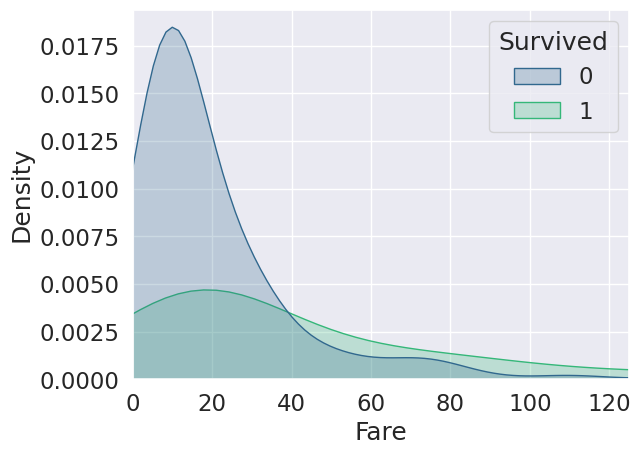
\includegraphics[width=0.49\linewidth]{fare.png}
    \end{subfigure}
    \caption{Distribution of numeric attributes with respect to target}
    \label{fig:enter-label}
\end{figure}
\paragraph{}From the distribution of the numeric attributes, it can be observed that a significant amount of children were in the group of survivors. The survivors also tend to have paid more for their tickets.
\newpage
\begin{figure}[htb]
    \centering
    \begin{subfigure}
        \centering
        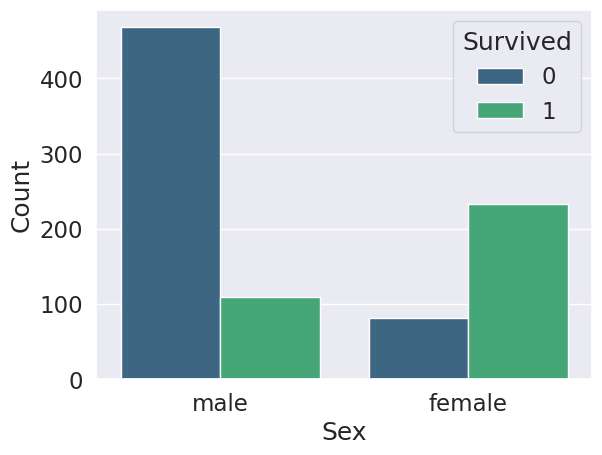
\includegraphics[width=0.49\linewidth]{sex.png}
    \end{subfigure}
    \begin{subfigure}
        \centering
        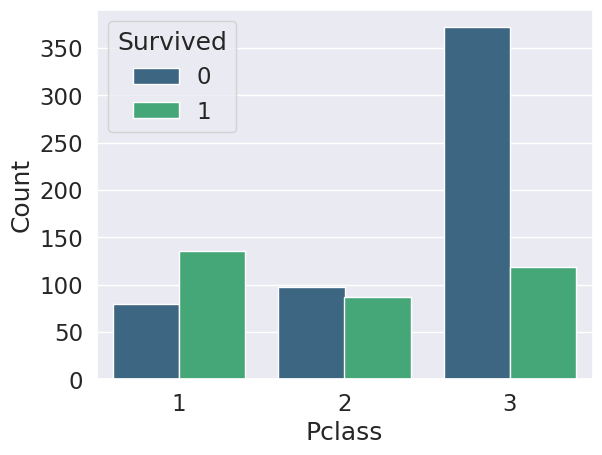
\includegraphics[width=0.49\linewidth]{pclass.png}
    \end{subfigure}
    \begin{subfigure}
        \centering
        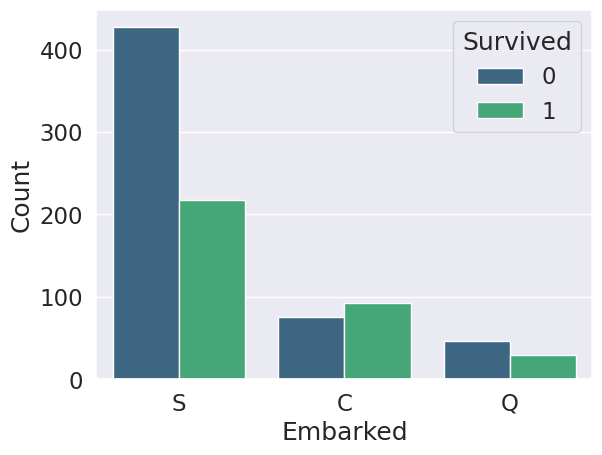
\includegraphics[width=0.49\linewidth]{embarked.png}
    \end{subfigure}
    \begin{subfigure}
        \centering
        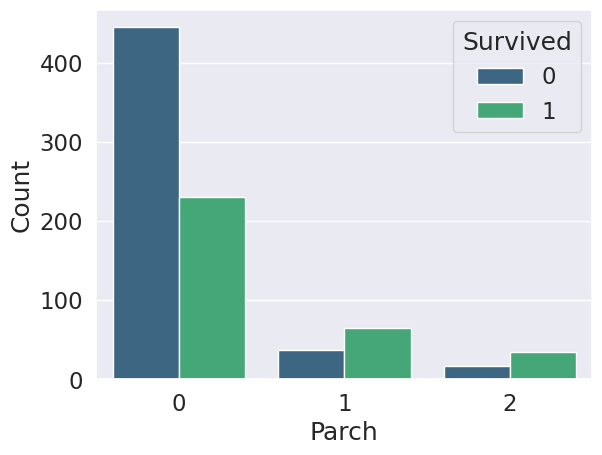
\includegraphics[width=0.49\linewidth]{parch.png}
    \end{subfigure}
    \begin{subfigure}
        \centering
        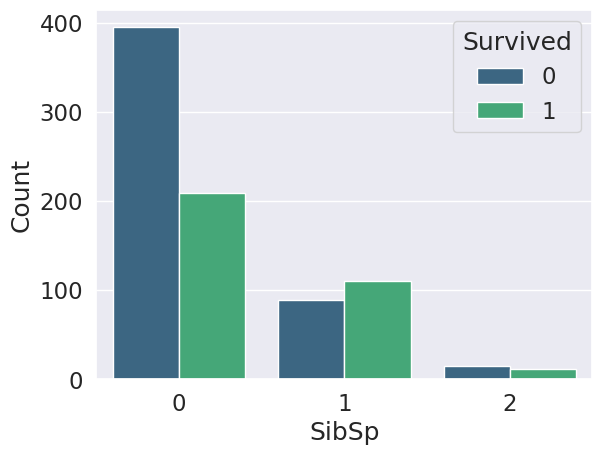
\includegraphics[width=0.49\linewidth]{sibsp.png}
    \end{subfigure}
    \caption{Distribution of categorical attributes with respect to target}
    \label{fig:enter-label}
\end{figure}

\paragraph{}From the distribution of categorical variables, it can be seen that most males and passengers of the 3rd class did not survive. Also, people with siblings/spouses and/or parents/children onboard were more likely to survive. The distribution of \textbf{Embarked} also shows that the port of departure may have had an influence on survival, however, these two attributes have very low correlation, so the statistics are most likely unrelated.
\newpage
\begin{figure}[htb]
    \centering
    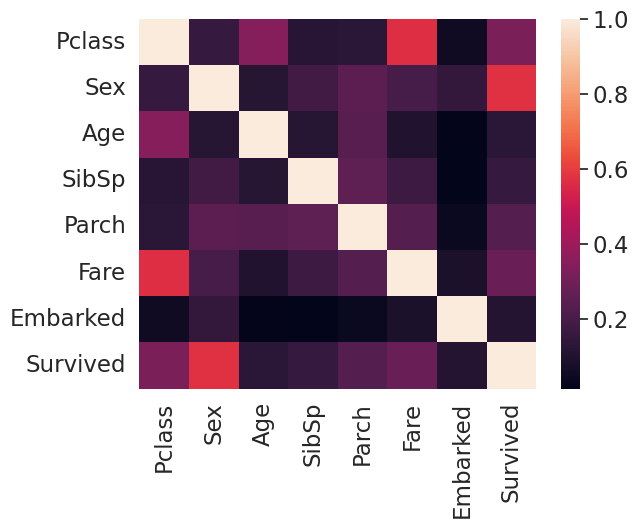
\includegraphics[width=0.75\linewidth]{corr_heatmap.png}
    \caption{Correlation matrix between input features and target}
    \small{(\textbf{Sex} and \textbf{Embarked} were encoded using integer values)}
    \label{fig:enter-label}
\end{figure}
\paragraph{}From the correlation matrix, it can be seen that the biggest factor in survival was the passenger's \textbf{Sex}, with \textbf{Pclass} having a significant influence as well. The only pair of input features, which can be considered highly correlated are \textbf{Pclass} and \textbf{Fare}.
\newpage
\section{Pre-processing techniques used}
\begin{itemize}
    \item \textbf{Drop PassengerId, Name and Ticket columns} - These features don't provide any useful information.
    \item \textbf{Impute missing values of Age with median grouped by Sex and Pclass, missing values of Embarked with the most common value and missing values of Fare with median} - This allows us to use the records with missing values in training our classifier, while assigning the most probable values to the missing attributes.
    \item \textbf{Classify missing values in Cabin as unknown} - The proportion of missing values in \textbf{Cabin} is so large that it may be beneficial for us to classify them as another possible value. With the previous insight that poorer passengers may not have been assigned cabins, it can give the model some more information.
    \item \textbf{Keep only the first character of Cabin} - The first character describes the deck level of each cabin, which is far more important than an individual cabin number.
    \item \textbf{Group the Cabin attribute into 4 clusters: Unknown, ABC, DE, FG} - Group similar passengers together.
    \item \textbf{One-hot encode the modified Cabin attribute, Embarked and Pclass} - Because these features have a high number of unique values, one-hot encoding them, as opposed to integer encoding, will help preserve their categorical nature.
    \item \textbf{Encode Sex as an integer} - This gives the classifier a numerical representation of this feature.
    \item \textbf{Introduce a new variable Family\_Size by combining SibSp and Parch} - This allows us to reduce the number of features.
    \item \textbf{Standard scaling of non-categorical columns} - This can help the classifier compare the passengers we are trying to classify to the passengers it learned from.
\end{itemize}
\newpage
\section{Output features}
\paragraph{}The classifier's task is to predict whether a given person survived the disaster or not, thus our model will output a single binary attribute.
\begin{figure}[htb]
    \centering
    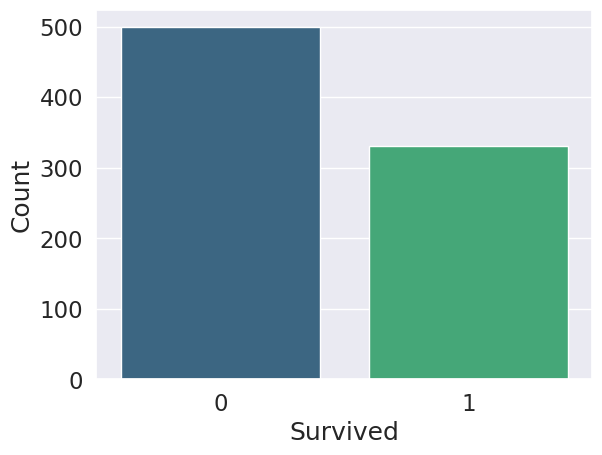
\includegraphics[width=0.85\linewidth]{target_distribution.png}
    \caption{Distribution of the target variable in the training dataset}
    \label{fig:enter-label}
\end{figure}
\paragraph{}The survival rate of passengers in the training data is equal to $38.\overline{38}\%$
\section{Conclusions}
\paragraph{}The aforementioned pre-processing techniques helped increase the classification accuracy of the model from \textbf{54.306\%} to \textbf{78.229\%}, which is a substantial increase. 

\end{document}